\begin{figure}[!htb]
    \begin{center}
        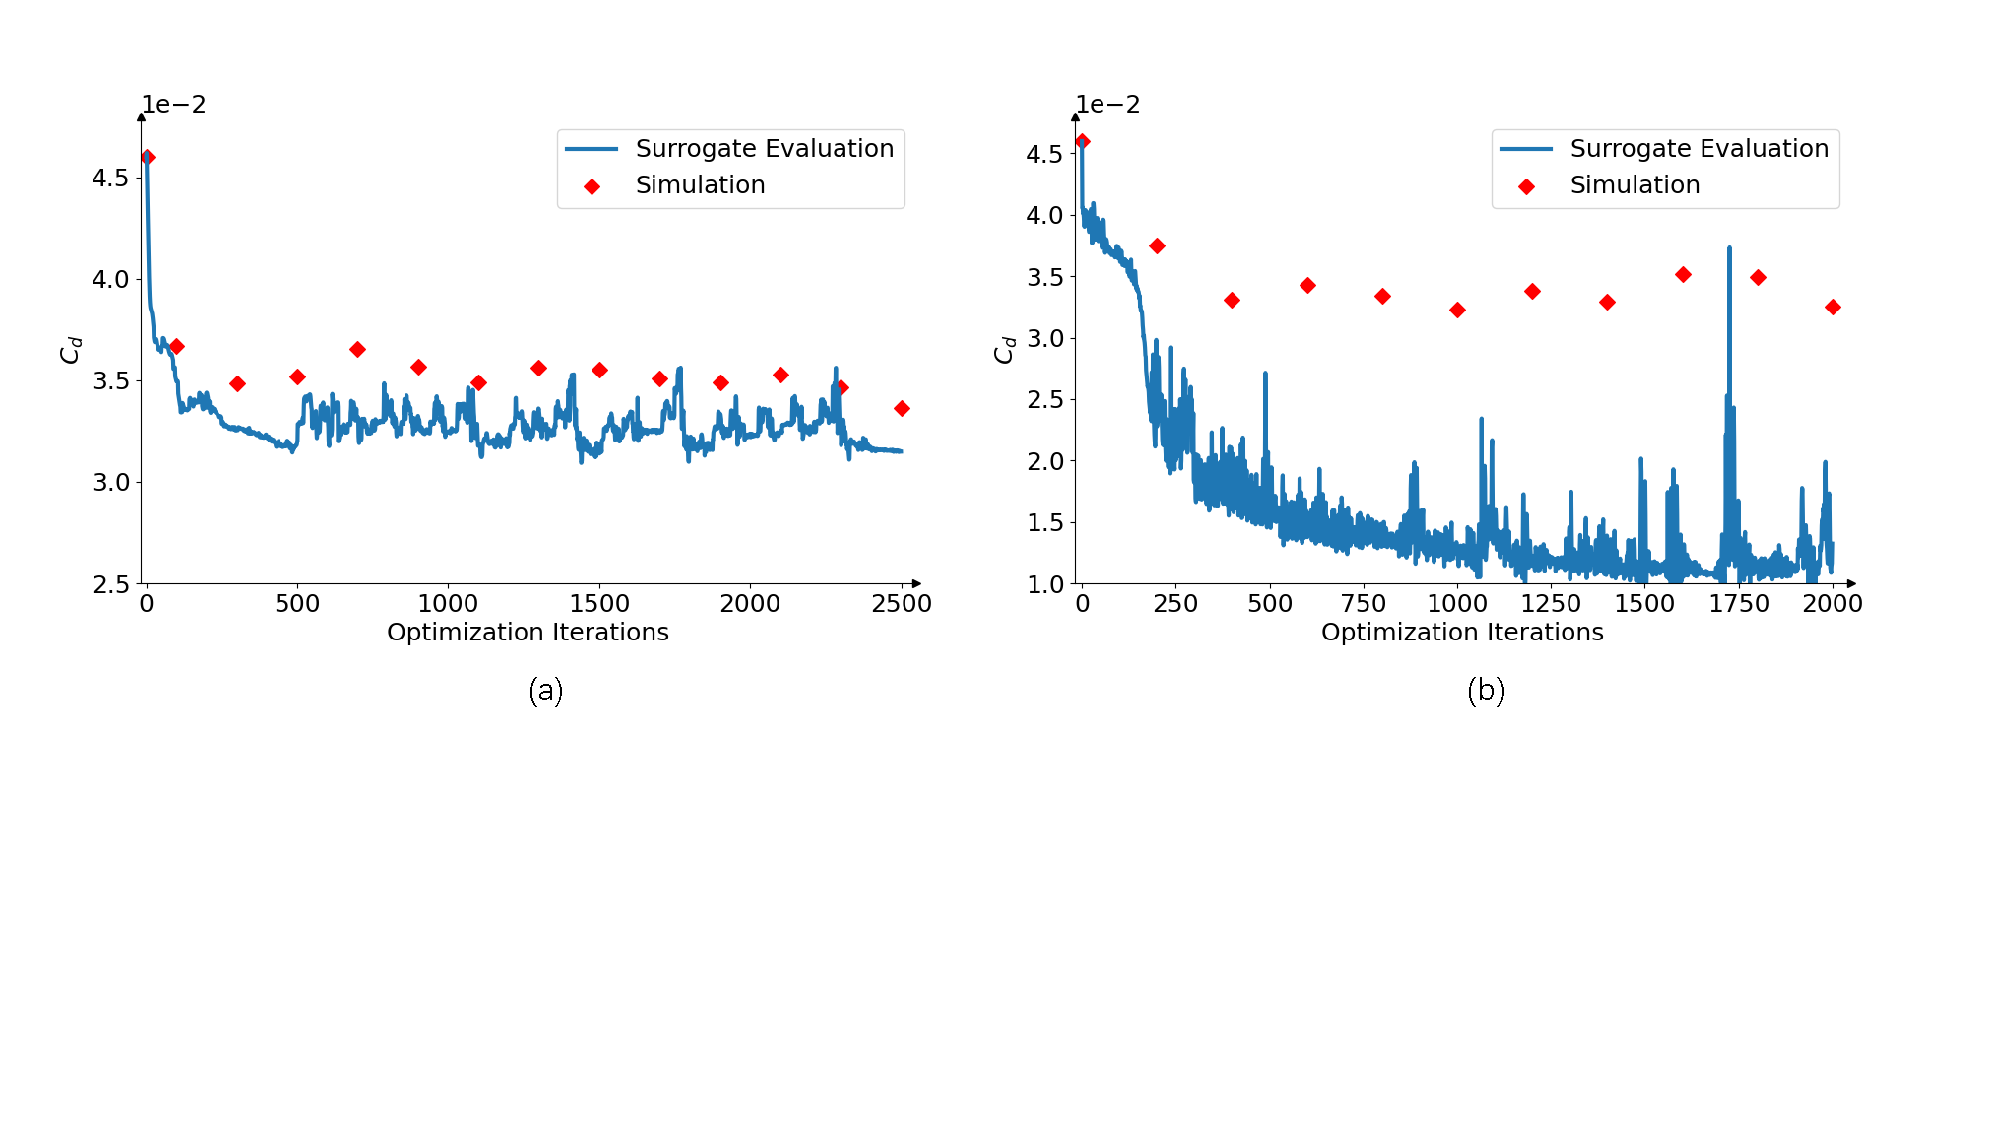
\includegraphics[width=0.9\linewidth]{chapter4/fig/lsm_dmm_gcnn_Cd_history.pdf}
    \end{center}
    \caption{
        \small The gap between GCNN's evaluations and simulation results becomes more significant when the airfoil is more deformed and falls outside the distribution of the training data, when it is combined with (a) LSM and (b) DMM. GCNN shows limited generalization ability when it only relies on a fixed training set.
    }
    \label{ch4:fig:gcnn_gap}
\end{figure}